\subsection{Configuración de conexiones}
Con Knex.js instalado, sólo falta configurar las conexiones.

Para realizar las configuraciones, se debe crear un archivo que lleve de preferencia el nombre ``knexfile.js''. En este archivo, se crea un objeto con las siguientes propiedades:
    \begin{itemize}
        \item alias: El nombre que se le dará a la conexión.
        \item client: El SGBD que se utilizará para realizar la conexión.
        \item connection: En esta propiedad se debe configurar lo siguiente:
            \begin{itemize}
                \item host: El servidor donde está almacenada la base de datos.
                \item port: El puerto donde se está ejecutando el SGBD.
                \item database: El nombre de la base de datos.
                \item user: El nombre del usuario dueño de la base de datos.
                \item password: La contraseña para acceder a la base de datos.
            \end{itemize}
        \item pool: En esta propiedad se debe configurar lo siguiente:
            \begin{itemize}
                \item min: El número mínimo de conexiones que se pueden realizar.
                \item max: El número máximo de conexiones que se pueden realizar.
                \item afterCreate: Una función que se ejecuta una vez realizada la conexión. Esta es opcional
            \end{itemize}
    \end{itemize}
La estructura del objeto queda de la siguiente manera:
    \begin{figure}[H]
        \begin{center}
            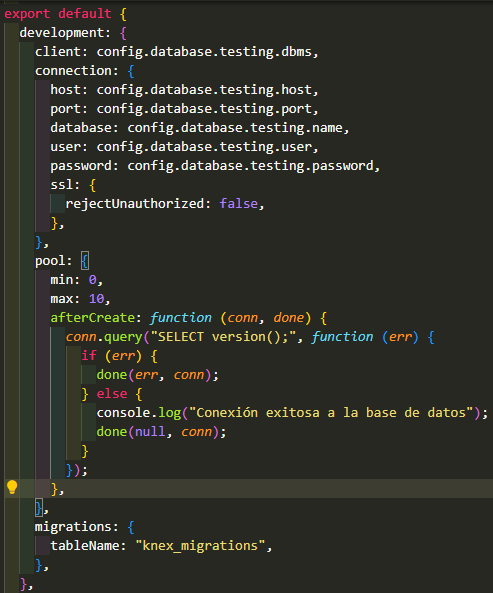
\includegraphics[scale=0.6]{img/actividades/conexion/objeto-conexion.png}
            \caption{Estructura del objeto de configuración de la conexión.}
            \label{fig:estructura-objeto}
        \end{center}
    \end{figure}
Por último, se crea una instancia de Knex y se le asigna la configuración que se desea utilizar, de esta manera se creará la conexión y se podrán realizar los queries que se requieran.